\documentclass[11pt,a4paper]{article}

\usepackage[spanish]{babel}
\usepackage[math,light]{iwona}
\usepackage[utf8]{inputenc}
\usepackage{amsmath, amsthm}
\usepackage{amsfonts, amssymb, latexsym}
\usepackage{enumerate}
\usepackage[usenames, dvipsnames]{color}
\usepackage{graphics,graphicx, float} %para incluir imágenes y colocarlas
\usepackage{colortbl}
\usepackage{graphicx}
\usepackage{wrapfig}
\usepackage[top=4cm]{geometry}
\usepackage{cite}
\usepackage[official]{eurosym}
\usepackage{cancel}
\usepackage{subfigure}
\usepackage{minted}

\theoremstyle{plain}
\newtheorem{exe}{Ejercicio} % reset theorem numbering for each chapter

\theoremstyle{definition}
\newtheorem{sol}{Solución}

\usepackage[bookmarks=true,
            bookmarksnumbered=false, % true means bookmarks in
                                     % left window are numbered
            bookmarksopen=false,     % true means only level 1
                                     % are displayed.
            colorlinks=true,
            linkcolor=webblue,
            citecolor=red]{hyperref}
\definecolor{webgreen}{rgb}{0, 0.5, 0} % less intense green
\definecolor{webblue}{rgb}{0, 0, 0.5}  % less intense blue
\definecolor{webred}{rgb}{0.5, 0, 0}   % less intense red

\setlength{\parindent}{0pt}
\setlength{\parskip}{1ex plus 0.5ex minus 0.2ex}

\newcommand{\HRule}{\rule{\linewidth}{0.5mm}}

\renewcommand\thesubsection{\alph{subsection}}

\title{\Huge{Visión por Computador} \\ Práctica 2}
\author{Marta Gómez Macías}

\begin{document}

\maketitle

\tableofcontents

\setcounter{section}{-1}
\section{Opción desarrollada}

Antes de empezar la práctica, aclarar que he escogido la \textbf{opción 1}.

\section{Detección de puntos Harris multiescala}

\subsection{Extraer puntos Harris a distintas escalas}

Para calcular los puntos \textit{Harris}, en primer lugar calculamos los autovalores de la imagen en cada escala, para ello, usamos la función \texttt{cornerEigenValsAndVecs} de \textit{OpenCV}, que nos devuelve una imagen con seis canales ($\lambda_1$, $\lambda_2$, $x_1$, $y_1$, $x_2$, $y_2$), donde:

\begin{enumerate}[$\bullet$]
\item $\lambda_1$ y $\lambda_2$ son los autovalores de $M$ no ordenados.

\item $x_1$ e $y_1$ son los autovectores de $\lambda_1$

\item $x_2$ e $y_2$ son los autovectores de $\lambda_2$
\end{enumerate}

Para calcular los puntos Harris usando \textit{\textbf{operador Harris}}, sólo necesitamos los autovalores de la matriz $M$. Dicho criterio es:

\begin{displaymath}
    f = determinant(M) - k \cdot trace(M)^2 = \lambda_1 \lambda_2 - k \cdot (\lambda_1 + \lambda_2)^2
\end{displaymath}

donde $k$ es una constante cuyo valor recomendado es $k = 0.04$. Si hubiésemos querido evitar usar la constante $k$ podríamos haber usado este otro criterio:

\begin{displaymath}
    f = \frac{\lambda_1 \lambda_2}{\lambda_1 + \lambda_2} = \frac{determinant(M)}{trace(M)}
\end{displaymath}

\begin{minted}[frame=lines, label={Operador de Harris}]{python}
# Función que implementa el criterio de Harris: det(M) - k * trace(M)
# este criterio también se puede expresar como: 
# lamba1*lambda2 / (lambda1+lambda2)^2 = det(M)/trace(M)^2
criterio_harris = lambda lambda1, lambda2, k=0.04: lambda1*lambda2 - \
                    k*((lambda1+lambda2)**2)
\end{minted}

Una vez tenemos el valor de \textit{Harris} de cada punto de la imagen, nos hacemos un pequeño filtro, para quedarnos con los puntos que dan un valor de \textit{Harris} más alto. Para hacer este filtro, creamos una imagen en color negro y ponemos en blanco los puntos cuyo valor de \textit{Harris} supera un determinado umbral, que dependerá de cada imagen. Para ello, usamos la función \texttt{binary\_harris}:

\begin{minted}[frame=lines, label={Implementación del filtrado con umbral}]{python}
# función que dada una matriz de harris y un umbral, devuelve una imagen 
# binaria donde los puntos blancos son los que superan dicho umbral
binary_harris = lambda matriz, umbral: (matriz >= umbral) * 255
\end{minted}

Todo el proceso que llevamos hecho hasta ahora puede resumirse en la siguiente función. El resultado de esta función puede verse en la \hyperref[umbral]{Figura \ref*{umbral}}, como se aprecia, más que puntos hemos obtenido ``zonas'' con un alto valor de \textit{Harris}. En cada zona, está el punto \textit{Harris} que buscamos y puntos que, al estar cerca de éste, tiene un valor de \textit{Harris} alto. 

\begin{minted}[frame=lines, label={Filtrando los puntos Harris con un umbral}]{python}
def create_binary_harris(lista_escalas, umbral):
    # y para cada escala, usamos la función de OpenCV "cornerEigenValsAndVecs" 
    # para extraer los mapas de auto-valores de la matriz Harris en cada píxel. 
    # Debemos tener en cuenta que esta función devuelve 6 matrices 
    # (lambda1, lambda2, x1, y1, x2, y2) donde:
    #       * lambda1, lambda2 son los autovalores de M no ordenados
    #       * x1, y1 son los autovectores de lambda1
    #       * x2, y2 son los autovectores de lambda2
    scale_eigenvalues = []  # lista de matrices en el que guardar resultados
    for escala in lista_escalas:
        scale_eigenvalues.append(cv2.cornerEigenValsAndVecs(src=escala, \
                                blockSize=3, ksize=3))

    # una vez tenemos los autovalores de cada imagen, creamos una matriz 
    # por cada escala con el criterio de harris
    matrices_harris = []  # lista de matrices para guardar las matrices 
                          # del criterio de harris para cada escala
    for escala in scale_eigenvalues:
        canales = cv2.split(escala) 
        matrices_harris.append(criterio_harris(lambda1=canales[0], lambda2=canales[1]))

    # inicializamos una lista de imágenes binarias a 255 si no supera un 
    # determinado umbral y a 255 si lo supera. Una por escala.
    binaria = [binary_harris(escala, umbral) for escala in matrices_harris]

    return binaria, matrices_harris
\end{minted}

\begin{figure}[!h]
    \centering
    \mbox{
        \subfigure[Imagen de prueba con muchas esquinas, que son los puntos que nuestro algoritmo debería detectar]{
        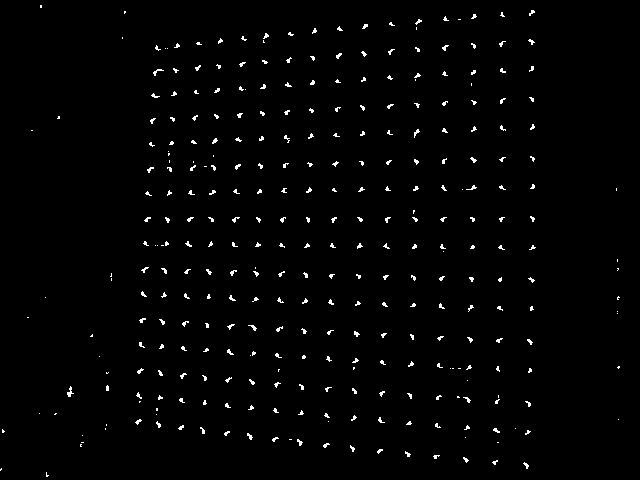
\includegraphics[width=0.5\textwidth]{img0}
        \label{umbralprueba}
        }

        \subfigure[Imagen de una montaña, con muchos cambios en los tonos de gris de la imagen]{
        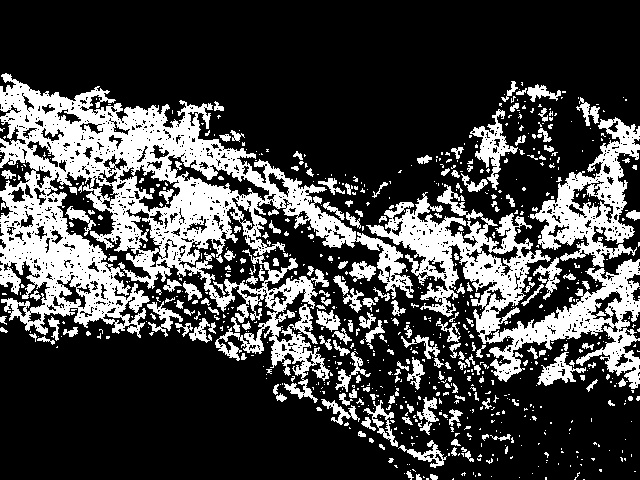
\includegraphics[width=0.5\textwidth]{img5}
        \label{umbralmont}
        }
    }
    \caption{Puntos cuyo valor de \textit{Harris} supera un determinado umbral}
    \label{umbral}
\end{figure}

Para poder eliminar todos los \textit{falsos máximos} implementamos la \textit{\textbf{supresión de no máximos locales}}. En la cual recorremos la imagen binaria con una ventana, si el centro de la ventana es un píxel en blanco comprobamos si es máximo local (usando la función \texttt{is\_localmax\_center}), en caso positivo pintamos de negro todos los píxeles de la ventana menos el central (usando la función \texttt{put\_zero\_least\_center}) y en caso negativo, pintamos el píxel central de negro.

\begin{minted}[frame=lines, label={Supresión de no máximos}]{python}
# función que tomando como entrada los valores de un entorno nos indica si 
# el valor del centro es máximo local. Estamos presuponiendo una ventana 2D 
#con un número impar de dimensiones (3x3, 5x5, etc)
is_localmax_center = lambda entorno: np.argmax(entorno) == floor(\
                    (entorno.shape[0]*entorno.shape[1])/2)

# función que pone en negro todos los píxeles de un entorno menos el central
def put_zero_least_center(img, window_size, i, j):
    img[i-window_size:i+window_size+1, j-window_size:j+window_size+1] = 0
    img[i,j] = 255
    
def remove_local_maxima(binaria, matrices_harris, window_size, scale):
    # una vez tenemos nuestra imagen binaria, la recorremos preguntando 
    # para cada posición con valor 255 si su correspondiente valor en 
    # la matriz de harris es máximo local o no.
    for escala in range(scale):
        # nos quedamos con los índices que superan el umbral
        harris_index = np.where(
            binaria[escala] == 255)  # where devuelve un vector con 
                                     # los índices fila y otro con las columnas
        # una vez tenemos esos indices, comprobamos si el valor de 
        # esa posición es máximo local o no
        for i in range(len(harris_index[0])):
            row = harris_index[0][i]
            col = harris_index[1][i]
            # comprobamos si el pixel row,col de la imagen binaria 
            # es máximo local
            if row >= window_size and col >= window_size and \
                is_localmax_center(matrices_harris[escala] \
                [row - window_size:row + window_size + 1,\
                col - window_size:col + window_size + 1]):
                # si es máximo local, ponemos en negro a todos los píxeles de su entorno
                put_zero_least_center(binaria[escala], window_size, row, col)
            else:
                # si no lo es, ponemos el píxel a 0
                binaria[escala][row, col] = 0
\end{minted}

\begin{figure}[!h]
    \centering
    \mbox{
        \subfigure[Una vez eliminados los no máximos, vemos cómo los puntos \textit{Harris} están en las esquinas de los cuadrados]{
        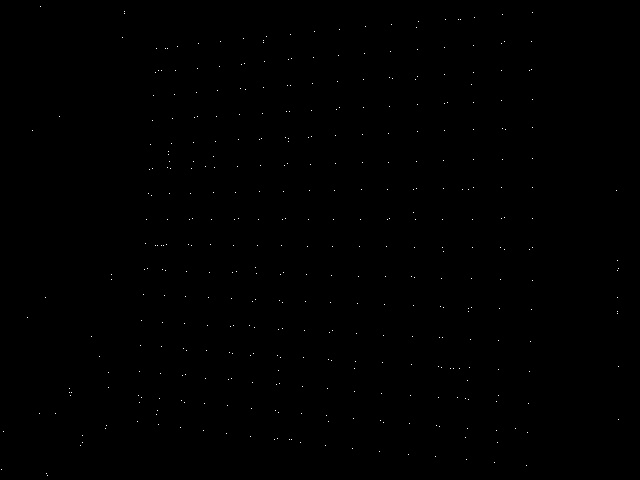
\includegraphics[width=0.5\textwidth]{img1}
        \label{maximosprueba}
        }

        \subfigure[Tras eliminar los no máximos, la imagen se ha quedado mucho más limpia]{
        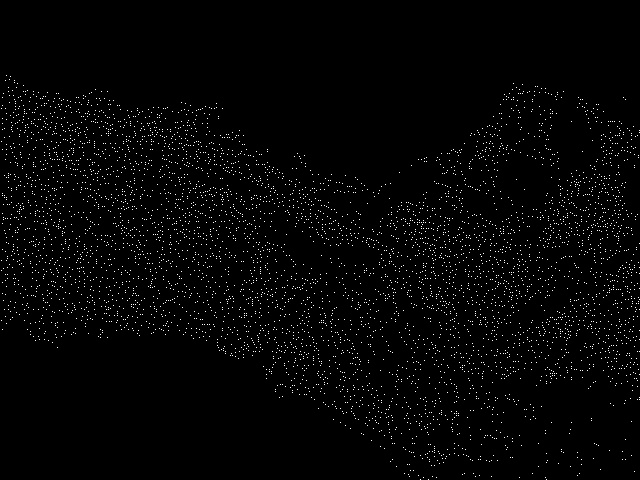
\includegraphics[width=0.5\textwidth]{img6}
        \label{maximosmont}
        }
    }
    \caption{Resultado tras eliminar los no máximos locales.}
    \label{maximos}
\end{figure}

En la \hyperref[maximos]{Figura \ref*{maximos}} vemos el resultado obtenido una vez hecha la supresión de no máximos. Si comparamos esta imagen con la anterior, se ve que hemos eliminado bastantes puntos y nos hemos quedado únicamente con los verdaderos máximos, con los puntos \textit{Harris}. 

El siguiente paso es quedarnos con los puntos que tengan un mayor valor de Harris y obviar el resto. Para ello, debemos ordenar los puntos por su valor de Harris y quedarnos con los $n$ primeros de la lista. Para poder trabajar de forma más sencilla, \texttt{numpy} nos proporciona herramientas para poder realizar filtrado y ordenación de elementos mediante sus índices.

\begin{minted}[frame=lines, label={Ordenando los puntos obtenidos}]{python}
def get_best_harris(matrices_harris, binaria, points_to_keep, n_points, scale):
    # una vez tenemos los puntos de Harris eliminando no máximos, los 
    # ordenamos por su valor de Harris para quedarnos con los n mejores
    best_harris = []
    for escala in range(scale):
        # nos quedamos con los índices que corresponden con puntos de harris
        harris_index = np.where(binaria[escala] == 255)
        # y también con el valor de harris de esos puntos
        harris_points = matrices_harris[escala][harris_index]
        # obtenemos los índices de los puntos del vector ordenados
        sorted_indexes = np.argsort(harris_points)[::-1]
        # juntamos en una matriz con dos columnas las coordenadas x,y de 
        # los puntos y nos quedamos con los n primeros
        best_harris.append(np.vstack(harris_index).T[sorted_indexes\
            [0:int(points_to_keep[escala] * n_points)]])
        binaria[escala][:] = 0
        binaria[escala][best_harris[escala][:, 0], \
            best_harris[escala][:, 1]] = 255

    return best_harris
\end{minted}

Una vez tenemos los mejores puntos \textit{Harris}, los representamos en la imagen. En la \hyperref[puntosfinal]{Figura \ref*{puntosfinal}} vemos el resultado final del método desarrollado. Como se aprecia, los puntos obtenidos se han colocado sobre esquinas de los cuadrados y puntos de la imagen donde se aprecia un cambio en la escala de grises. Por tanto, podemos concluir que el método ha obtenido unos buenos resultados.

\begin{figure}[!h]
    \centering
    \mbox{
        \subfigure[En este caso hemos obtenido pocos puntos, por lo que no hemos eliminado ningun punto \textit{Harris} al ordenar]{
        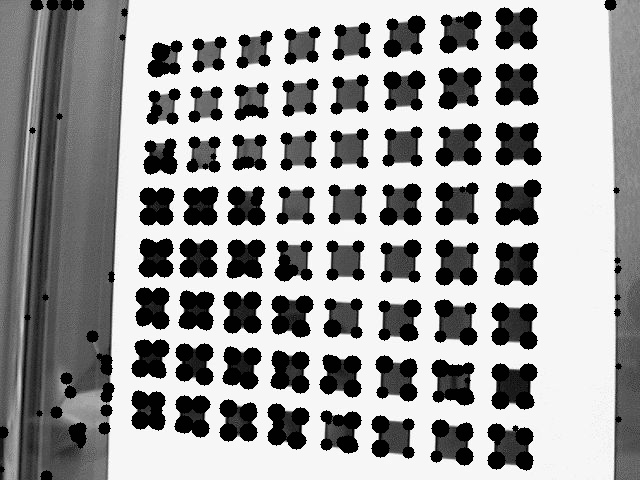
\includegraphics[width=0.5\textwidth]{img2}
        \label{puntosfinalprueba}
        }

        \subfigure[En cambio, en este caso hemos eliminado muchísimos puntos, quedándonos con los que están sobre picos y laderas con un fuerte contraste]{
        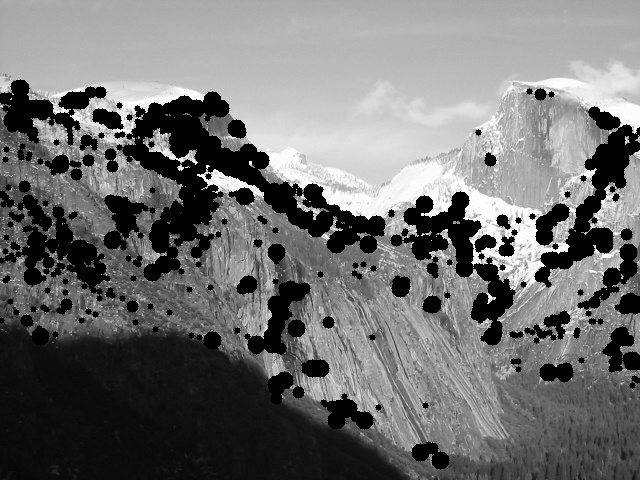
\includegraphics[width=0.5\textwidth]{img7}
        \label{puntosfinalmont}
        }
    }

    \caption{Puntos \textit{Harris} obtenidos representados sobre la imagen original}
    \label{puntosfinal}
\end{figure}

\newpage
\subsection{Refinar la posición de los puntos a nivel de sub-píxel}

Para hacer este apartado, es necesario usar la función de \textit{OpenCV} \texttt{cornerSubPix}. Al estar trabajando a nivel de sub-píxel, esta función necesita trabajar con datos flotantes.

\begin{minted}[frame=lines, label={Refinamiento a nivel de sub-píxel}]{python}
# Función para refinar las esquinas sacadas en el apartado a con conrnerSubPix
def refina_Harris(escalas, esquinas, scale=3):
    ref_escalas = []
    for i in range(len(escalas)):
        float_esquinas = np.array(esquinas[i], dtype=np.float32)
        cv2.cornerSubPix(image=escalas[i], corners=float_esquinas, \
            winSize=(5,5), zeroZone=(-1,-1), \
            criteria=(cv2.TERM_CRITERIA_MAX_ITER | cv2.TERM_CRITERIA_COUNT, 10, 0.01))
        ref_escalas.append(float_esquinas)

    draw_circle_on_corners(img=escalas[0], esquinas=ref_escalas,scale=scale)
    return ref_escalas
\end{minted}

\begin{figure}[!h]
    \centering
    \mbox{
        \subfigure[Debido al truncamiento a la hora de representar los puntos, hemos obtenido algunos que están en zonas planas]{
        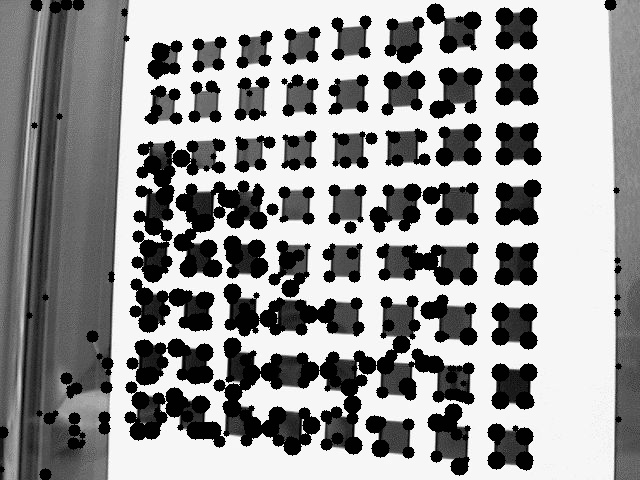
\includegraphics[width=0.5\textwidth]{img3}
        \label{refpuntosfinalprueba}
        }

        \subfigure[En este caso no se aprecian muchas diferencias visibles con el anterior resultado]{
        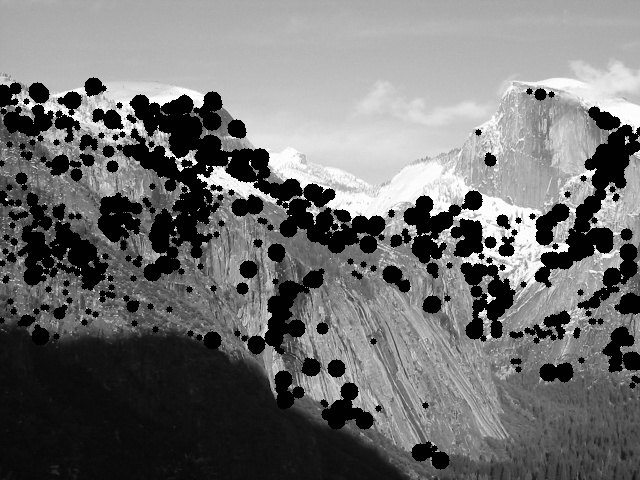
\includegraphics[width=0.5\textwidth]{img8}
        \label{refpuntosfinalmont}
        }
    }

    \caption{Refinamiento a nivel de sub-píxel de los puntos \textit{Harris} obtenidos representados sobre la imagen original}
    \label{refpuntosfinal}
\end{figure}

En la \hyperref[refpuntosfinal]{Figura \ref*{refpuntosfinal}} vemos el resultado de esta función. Pienso que no se puede apreciar el resultado en la imagen, ya que a la hora de representar los puntos en la misma se hace un truncamiento para calcular el centro del círculo y por tanto, obtenemos puntos cuyo centro es una zona plana de la imagen.

\subsection{Calcular la orientación de los puntos Harris}

Para calcular la orientación de un punto, debemos calcular los gradientes en $x$ y en $y$ aplicando derivadas en los ejes $x$ e $y$ de las imágenes. Para ello, aplicamos un kernel gaussiano con $\sigma = 4,5$ a la imagen en un sólo eje ($x$ o $y$). Una vez tenemos las derivadas, calculamos la orientación $\theta$ en cada punto con la siguiente fórmula:

\begin{displaymath}
\theta_{xy} = arctan \Bigg ( \frac{grad_y}{grad_x} \Bigg)
\end{displaymath}

El vector correspondiente a la orientación $\theta$ es $[cos(\theta), sin(\theta)]$. 

Un detalle de implementación de la función, es que sólo calculamos la arcotangente de los puntos Harris, ya que son los que nos interesan.

\begin{minted}[frame=lines, label={Cálculo de la orientación de cada punto Harris}]{python}
# Función para calcular la orientación de cada esquina encontrada.
def find_orientacion(escalas, esquinas, sigma=4.5):
    # calculamos las derivadas en x y en y aplicando un filtro sobel sobre 
    # la imagen. Una vez calculadas las derivadas, calcular la arcotangente, 
    # que será la orientación del punto.
    orientaciones = []
    for i in range(len(escalas)):
        k = my_getGaussianKernel(sigma=sigma)
        esq_int = esquinas[i].T.astype(int)
        grad_x = my_filter2D(src=escalas[i], kernel=k, borderType='reflect',\
                             ejex=True, ejey=False)[esq_int[0], esq_int[1]]
        grad_y = my_filter2D(src=escalas[i], kernel=k, borderType='reflect',\
                             ejex=False, ejey=True)[esq_int[0], esq_int[1]]
        orientaciones.append(np.arctan2(grad_y, grad_x))

    draw_circle_on_corners(img=escalas[0], esquinas=esquinas, scale=3, \
        orientaciones=orientaciones, addOrientation=True)

    return orientaciones
\end{minted}

\begin{figure}[!h]
    \centering
    \mbox{
        \subfigure[Orientaciones obtenidas para la imagen de prueba]{
        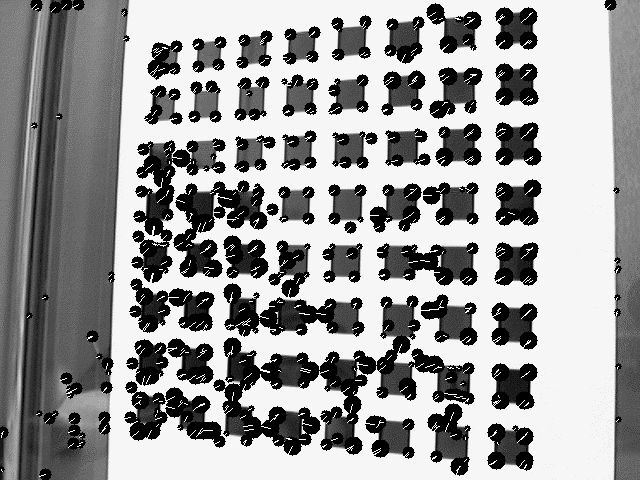
\includegraphics[width=0.5\textwidth]{img4}
        \label{orprueba}
        }

        \subfigure[Orientaciones obtenidas para la imagen de Yosemite]{
        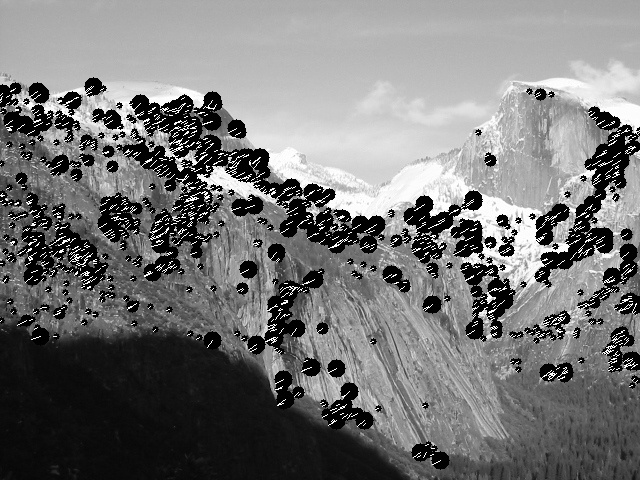
\includegraphics[width=0.5\textwidth]{img9}
        \label{ormont}
        }
    }

    \caption{Representación de la orientación de cada punto sobre la imagen original}
    \label{or}
\end{figure}

En la \hyperref[or]{Figura \ref*{or}} vemos el resultado obtenido por esta función, creo que está bien calculado ya que obtengo una orientación diferente en cada punto de las imágenes.

\section{Establecer correspondencias entre dos imágenes}

Para ello, vamos a usar el detector de \textit{OpenCV} \textbf{AKAZE}. Con dicho detector, vamos a extraer una lista de \texttt{keyPoints} y un descriptor por cada imagen (en este caso sólo usaremos dos imágenes). Para poder usar el criterio de correspondencias \textbf{BruteForce + crossCheck}, debemos usar los métodos de la clase \texttt{BFMatcher} con el flag \texttt{crossCheck} activado. Además, para calcular las distancias entre puntos usaremos la ditancia euclídea (parámetro \texttt{NORM\_L2}):

\begin{displaymath}
 |x| = \sqrt{\sum_{k=1}^n |x_k|^2} 
\end{displaymath}

Con el flag \texttt{crossCheck} activado, el método \texttt{knnMatch} con $k=1$ nos devolverá las parejas $(i,j)$ tales que $i$ sea el descriptor más cercano para $j$ y viceversa. De todas las parejas que nos devuelve este método, debemos quedarnos con las $n$ mejores.

\begin{minted}[frame=lines, label={Cálculo de las correspondencias entre dos imágenes}]{python}
def knn_matching(bf, desc1, desc2, kps1, kps2, img1, img2, n, k=1):
    # como crossCheck es True, knnMatch con k = 1 nos devolverá las parejas 
    #(i,j) tales que el vecino más cercano de i sea j y viceversa
    matches = bf.knnMatch(desc1, desc2, k=1)

    # tomamos n aleatorios para dibujarlos
    indices = sample(range(len(kps2)), n)

    matches_img = cv2.drawMatchesKnn(img1=img1, keypoints1=kps1, img2=img2, \
                keypoints2=kps2, matches1to2=[matches[i] for i in indices], \
                outImg=None)
    mostrar(matches_img)

def normal_matching(bf, desc1, desc2, kps1, kps2, img1, img2, n):
    matches = bf.match(desc1, desc2)

    # tomamos n aleatorios para dibujarlos
    indices = sample(range(len(kps2)), n)

    # dibujamos los n primeros
    matches_img = cv2.drawMatches(img1=img1, keypoints1=kps1, img2=img2, \
                keypoints2=kps2, matches1to2=[matches[i] for i in indices],\
                outImg=None)
    mostrar(matches_img)

    return matches

def akaze_match(img1, img2, n=50):
    # pasamos las fotos a blanco y negro
    gray1 = cv2.cvtColor(img1, cv2.COLOR_BGR2GRAY)
    gray2 = cv2.cvtColor(img2, cv2.COLOR_BGR2GRAY)

    # inicializamos el descriptor AKAZE
    detector = cv2.AKAZE_create()

    # detectamos los keypoint y extraemos los descriptores de ambas fotos. 
    # El parámetro None es debido a que no usamos ninguna máscara
    kps1, descs1 = detector.detectAndCompute(image=gray1, mask=None)
    kps2, descs2 = detector.detectAndCompute(image=gray2, mask=None)

    # dibujamos los puntos claves en la imagen 1
    keypoints_img1 = cv2.drawKeypoints(image=gray1, keypoints=kps1, \
                    outImage=None, color=(0,0,255), \
                    flags=cv2.DRAW_MATCHES_FLAGS_DRAW_RICH_KEYPOINTS)
    mostrar(keypoints_img1)
    # y en la imagen 2
    keypoints_img2 = cv2.drawKeypoints(image=gray2, keypoints=kps2, \
                    outImage=None, color=(255, 0, 0),\
                    flags=cv2.DRAW_MATCHES_FLAGS_DRAW_RICH_KEYPOINTS)
    mostrar(keypoints_img2)

    # para hacer el matching, usamos la fuerza bruta y validación cruzada, 
    # NORM_L2 es la distancia euclídea.
    bf = cv2.BFMatcher(normType=cv2.NORM_L2, crossCheck=True)

    # hacemos el matching usando knn
    knn_matching(bf=bf, desc1=descs1, desc2=descs2, kps1=kps1, kps2=kps2, \
                img1=img1, img2=img2, n=n)

    # hacemos el matching usando el método match
    matches = normal_matching(bf=bf, desc1=descs1, desc2=descs2, kps1=kps1, \
                    kps2=kps2, img1=img1, img2=img2, n=n)

    return matches, kps1, kps2

\end{minted}

\begin{figure}[!h]
    \centering
    \subfigure[Correspondencias obtenidas con \texttt{knnMatch}]{
    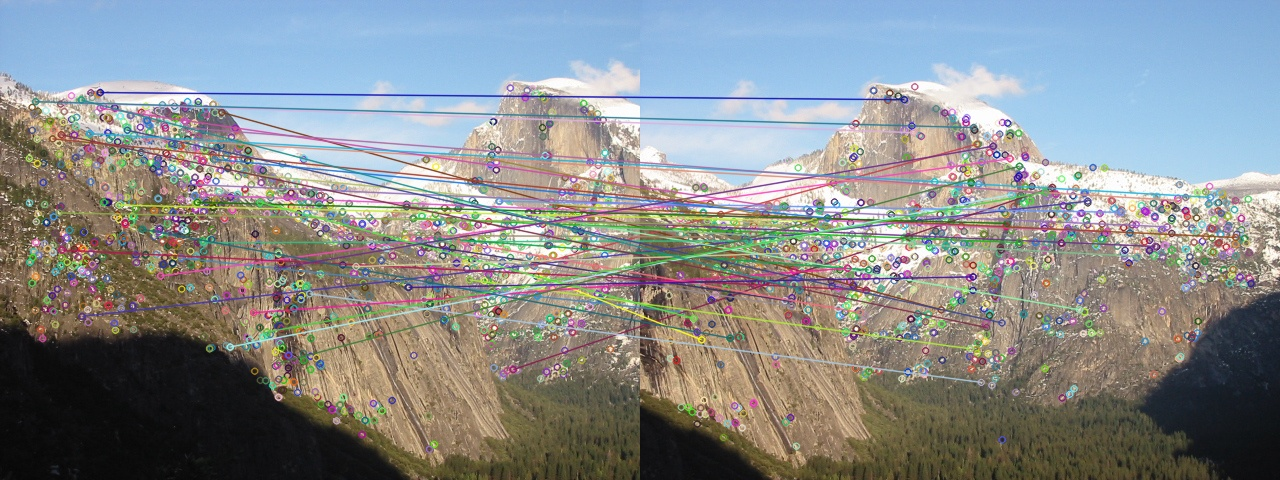
\includegraphics[width=\textwidth]{img12}
    \label{corknn}
    }
    \subfigure[Correspondencias obtenidas con \texttt{match}]{
    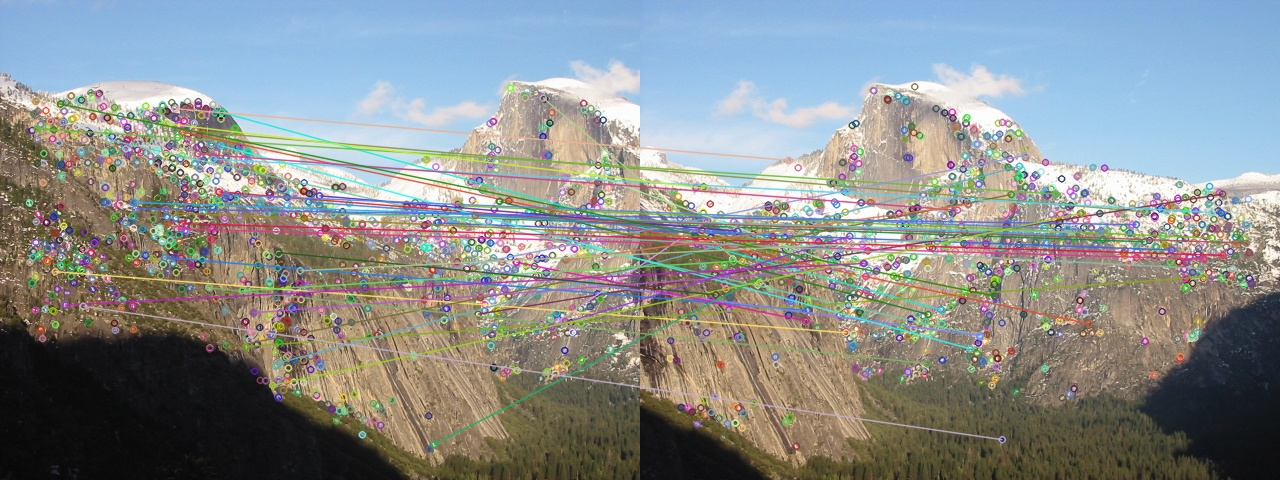
\includegraphics[width=\textwidth]{img13}
    \label{cornmat}
    }
    \caption{Correspondencias obtenidas entre las dos imágenes}
    \label{correspondencias}
\end{figure}

En la \hyperref[correspondencias]{Figura \ref*{correspondencias}} vemos el resultado de esta función. Como se ve, algunas correspondencias sí que son correctas, en cambio, también ha hecho correspondencias con puntos de una imagen que no aparecen en la otra y por tanto, son erróneos. Esto se debe a que las zonas en las que se ha hecho la correspondencia errónea son muy similares entre sí.

En general, vemos que hay líneas rectas pero también líneas en otras direcciones. Este es el resultado que esperábamos, ya que es imposible que este método calcule las correspondencias correctamente al 100\%. Además, he hecho las correspondencias usando dos métodos: \texttt{knnMatch} y \texttt{match}, con ambas obtengo un resultado prácticamente idéntico.

\section{Crear un mosaico}

\subsection{Crear un mosaico con dos imágenes}

Para crear un mosaico entre dos imágnenes me apoyo principalmente en dos funciones de \textit{OpenCV}: \texttt{findHomography} y \texttt{warpPerspective}. La primera la uso para calcular la homografía con la que relaciono ambas imágenes y la segunda, para transformar la segunda imagen (usando la homografía $H$ calculada anteriormente) de forma que pueda encajar con la primera en el plano del mosaico.

\begin{minted}[frame=lines, label={Haciendo un mosaico con dos imágenes}]{python}
def mosaico_dos(img1, img2, epsilon=0.5, mostrar_img=True):
    matches, kps1, kps2 = akaze_match(img1=img1, img2=img2, mask=None, 
                            mostrar_img=False)

    puntos_dst = np.float32([kps1[m.queryIdx].pt for m in \
                matches]).reshape(-1, 1, 2)

    puntos_src = np.float32([kps2[m.trainIdx].pt for m in \
                matches]).reshape(-1,1,2)

    homografia, mascara = cv2.findHomography(srcPoints=puntos_src, 
                        dstPoints=puntos_dst, method=cv2.RANSAC,
                        ransacReprojThreshold=epsilon)

    result = cv2.warpPerspective(src=img2, M=homografia, 
            dsize=(img1.shape[1] + img2.shape[1], img2.shape[0]))

    result[0:img1.shape[0], 0:img1.shape[1]] = img1

    result=np.delete(arr=result, obj=np.where(result==0)[1],axis=1)

    if mostrar_img:
        mostrar(result)

    return result
\end{minted}

\begin{figure}[!h]
    \centering
    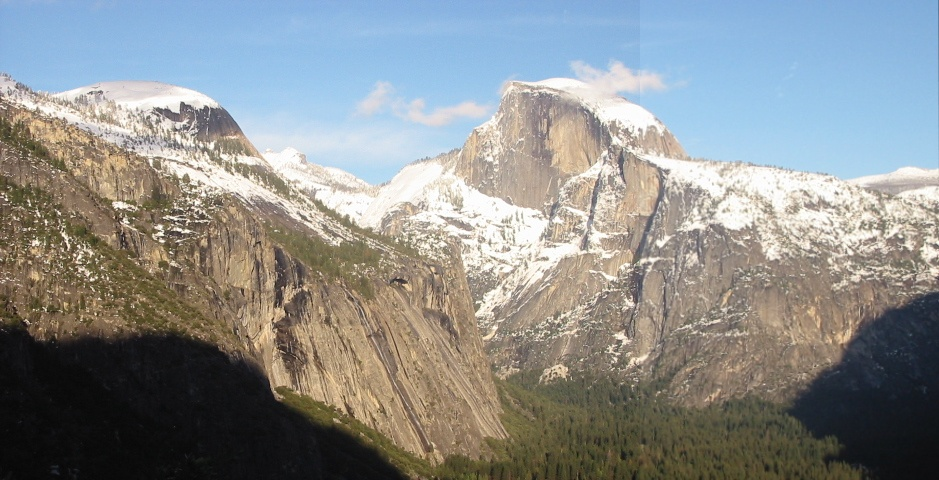
\includegraphics[width=0.7\textwidth]{img14}
    \caption{Mosaico con dos imágenes}
    \label{dosimagenes}
\end{figure}

Como se ve en la \hyperref[dosimagenes]{Figura \ref*{dosimagenes}}, el mosaico obtenido encaja perfectamente y lo único que puede resultar extraño es el cambio en el azul del cielo: en la primera imagen el color es más intenso que en la segunda. Para corregir esto tendríamos que hacer un degradado entre ambos azules de forma que el cambio no fuese tan brusco y no resultase tan extraño al ojo.

\subsection{Mosaico entre $n$ imágenes}

Para calcular un mosaico entre varias imágenes, he decidido aprovechar la función que he hecho para hacerlo entre dos. Mi función funciona de la siguiente manera: en primer lugar divido la lista de imágenes en dos, y \textit{\textbf{recursivamente}}, hago un mosaico de cada una de las mitades de la lista de imágenes. Esto lo hago para obtener la menor deformación posible en la imagen final. Si empezase a hacer mosaicos por uno de los extremos de la lista, el extremo contrario quedaría totalmente deformado y obtendríamos un mosaico \textit{estéticamente más feo}.

\begin{minted}[frame=lines, label={Mosaico con n imágenes}]{python}
# mosaico con más de dos imágenes asumiendo que las pasamos 
# al programa en orden
def mosaico_n(lista_imagenes):
    if len(lista_imagenes) == 3:
        # hacemos un mosaico con las dos primeras imagenes
        mosaico_12 = mosaico_dos(img1 = lista_imagenes[0], 
                    img2=lista_imagenes[1], mostrar_img=False)

        mosaico_23 = mosaico_dos(img1 = lista_imagenes[1], 
                    img2=lista_imagenes[2], mostrar_img=False)
        # y los unimos
        return mosaico_dos(img1=mosaico_12, img2=mosaico_23, mostrar_img=False)

    elif len(lista_imagenes) == 2:
        return mosaico_dos(img1=lista_imagenes[0], img2=lista_imagenes[1], 
                        mostrar_img=False)

    else:
        # nos quedamos con el índice de la imagen central
        central = floor(len(lista_imagenes)/2)
        # llamamos recursivamente a esta función con dos listas
        mosaico_primeramitad = mosaico_n(lista_imagenes[:central])
        mosaico_segundamitad = mosaico_n(lista_imagenes[central:])
        # y hacemos un mosaico con ambas
        mosaico = mosaico_dos(img1=mosaico_primeramitad, 
                    img2=mosaico_segundamitad, mostrar_img=False)

        mostrar(mosaico)

        return mosaico
\end{minted}

\begin{figure}[!h]
    \centering
    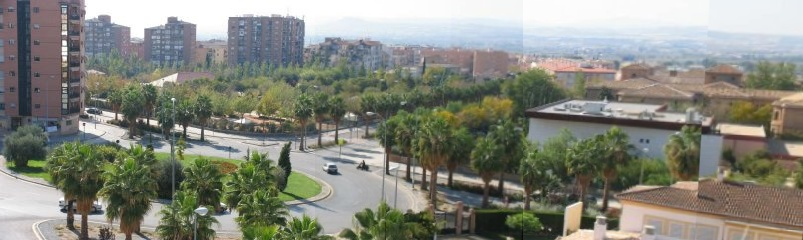
\includegraphics[width=0.7\textwidth]{img17}
    \caption{Mosaico con $n$ imágenes}
    \label{nimagenes}
\end{figure}

En la \hyperref[nimagenes]{Figura \ref*{nimagenes}} vemos un mosaico obtenido con esta función. La calidad general del mosaico obtenido es buena. Sin embargo, en la segunda mitad del mosaico vemos que la última imagen no se ha acoplado bien del todo. Esto se debe a que entre la imagen \textit{mosaico009.jpg} y \textit{mosaico010.jpg} hay un cambio de altura y la homografía entre estas dos imágenes no se ha calculado correctamente.

Además, no se ve en el mosaico toda la imagen \textit{mosaico011.jpg} debido a que la altura del mosaico es la misma que la altura de la primera imagen y además, se recorta toda la parte en negro.

\end{document}